\section{Introduzione}
\subsection{Considerazioni iniziali}
\subsubsection{Che cos'è Internet?}
Internet è... dipende da quale punto di vista lo si guarda:
\begin{itemize}
    \item Da un punto di vista \emph{pragmatico} Internet è un sistema che unisce milioni di calcolatori, detti \emph{host} sui quali girano applicazioni. Comprende inoltre \emph{link di connessione} (cioè fibra ottica, cavi in rame, connessioni radio e satellitari) che trasmettono con un certo rateo detto \emph{bandwith}. In fine comprende i \emph{router}, elementi che si occupano di fare indirizzamento dei pacchetti tra sottoreti diverse. Per funzionare usa dei protocolli, cioè delle regole per trasmettere e ricevere. Queste regole sono standardizzate da enti come IEEE, IETF, ecc tramite i RFC (Request For Comments)
    
    \item Da un punto di vista ad alto livello è una infrastruttura di comunicazione che ci permette di avere applicazioni distribuite utilizzando le API che mette a disposizione:
    \begin{itemize}
        \item trasferimento affidabile da sorgente a destinatario
        \item trasmissione \emph{best effort} ma non affidabile
    \end{itemize}
\end{itemize}

\subsubsection{Che cos'è un protocollo?}
\emph{Definisce il formato, l'ordine dei messaggi inviati e ricevuti tra elementi della rete e le azioni da intraprendere alla ricezione o invio di un messaggio}


\subsection{Componenti della rete}
Possiamo scomporre la rete in 3 porzioni principali:
\begin{itemize}
    \item Network edge: è composta dai calcolatori, detti \emph{host} e le loro applicazioni.
    \item Access network: sono le componenti che mettono in connessione gli host attraverso i \emph{link di connessione} (cablata, wireless, ecc).
    \item Network core: sono le connessioni tra le varie reti di accesso. E' la rete delle reti.
\end{itemize}

\subsubsection{Network edge}
Il focus principale della rete è permettere la comunicazione tra processi, quindi tra applicazioni. Le reti permettono di avere due architetture per le applicazioni:
\begin{itemize}
    \item Client/Server: un client è un host che richiede un servizio, un server è un host che fornisce un servizio. Si noti che la nomenclatura client/server si riferisce ai processi ma spesso si usa anche per indicare la macchina stessa che ospita il processo.
    
    Il browser è un processo client, il server web è un processo server.
    
    \item Peer to peer: ogni host può essere sia client che server in momenti diversi o allo stesso momento.
    
    BitTorrent è client mentre scarica, è un server quando fa da seed per altri host.
\end{itemize}


\subsubsection{Reti di accesso}
Le reti di accesso connettono i dispositivi tra di loro ed alla rete, le classifichiamo in:
\begin{itemize}
    \item \emph{reti di accesso residenziale}: ad esempio una rete domestica
    \item \emph{reti di accesso istituzionali}: ad esempio una rete universitaria
    \item \emph{reti di accesso mobile}: come ad esempio la rete 4G
\end{itemize}


\subsubsection{Media}
Per connettere i dispositivi tra di loro si usano i \emph{media} fisici:
\begin{itemize}
    \item Twisted pairs: doppino telefonico e cavo ethernet. Sono coppie di fili in rame isolati singolarmente ed avvolti l'uno con l'altro. Ne abbiamo di vari tipi in base all'isolamento: Unshielded twisted pairs, shielded twisted pairs, screened twisted pairs. Un filo serve per ricevere ed un altro serve per inviare.
    
    \item Coaxial cable: due conduttori cilindrici concentrici, è usato per la televisione ma nei primi anni della rete è stato usato come media. E' bidirezionale ed è in rame.
    
    \item Fibra ottica: sfrutta la propagazione della luce in un mezzo, codifica i bit in impulsi luminosi. Permette alti bitrate ed un tasso di errore molto basso anche dovuto all' immunità al rumore elettromagnetico.
    
    \item Radio: il segnale è trasportato (carried) su spettro elettromagnetico. E' bidirezionale. Potrebbero esserci problemi di propagazione quali riflessione, ostruzione dovuta agli oggetti o interferenze elettromagnetiche.
    E' un mezzo \emph{unguided} in quanto quando si emette lo si fa più o meno in tutte le direzioni. Ci sono diversi tipi di comunicazioni radio tra le quali citiamo: WiFi, wide-area (3G, 4G) e satellitare.
\end{itemize}

\subsubsection{Network Core}
E' una mesh di reti interconnesse. I dati all'interno della rete possono essere mossi in due modi:
\begin{itemize}
    \item Circuit switching
    \item Packet switching
\end{itemize}

\subsection{Tipologie di reti di accesso}

\subsubsection{Reti Dial-up}
Uno dei primi modi di connettersi alla rete prevedeva l'uso della rete telefonica già esistente. Si usava un modem che trasformava i bit in segnali che potevano essere trasmessi sulla rete dei doppini telefonici verso i router del provider. La connessione permetteva di viaggiare fino a 56 kbps e non permetteva di utilizzare il telefono domestico in contemporanea.

\begin{figure}[H]
    \centering
    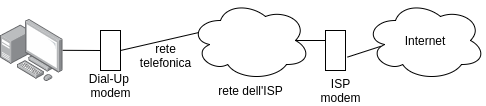
\includegraphics[width=330px]{images/1_Introduzione/dial-up.png}
\end{figure}

\subsubsection{Reti DSL}
DSL - Digital Subscriber Line utilizza le moderne reti telefoniche che permettono comunicazioni con larghezza di banda più grande (bandwith). E' una rete dedicata quindi permette di utilizzare sia internet che la rete telefonica allo stesso tempo. Utilizza media in rame. La versione più comune nelle abitazioni è ADSL in cui A sta per asimmetrico in quanto la velocità di upload (\emph{uplink}) è diversa dalla velocità di download (\emph{downlink}).

\begin{figure}[H]
    \centering
    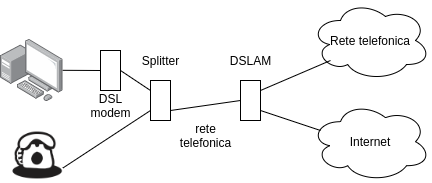
\includegraphics[width=330px]{images/1_Introduzione/DSL.png}
\end{figure}

\subsubsection{Rete via cavo}
Negli Stati Uniti è molto diffusa la televisione via cavo (a differenza dell'Italia che usa le trasmissioni via radio) quindi l'infrastruttura esistente è stata molto usata per dare connessione ad internet. La rete è condivisa con molti altri utenti usando una divisione in canali del mezzo.

\subsubsection{Fiber to the Home}
I media usati sono in fibra ottica e nelle case si pone un modem per modulare i bit in segnali luminosi da far arrivare all'ISP.

\subsubsection{Ethernet access}
Sono le reti più diffuse, si pone uno switch al centro della rete al quale si connettono vari host, in fine questo switch si connette al router che porta all'ISP. Oggi giorno un modello di questo tipo è presente in tutte le case poiché i modem domestici si compongono anche di switch e router.

\subsubsection{Wireless network}
Sono le reti wireless, si pone un access point al quale si connettono i dispositivi che permettono connessioni wireless. Anche qui ci vuole un router per far arrivare il traffico all'ISP.

\subsection{Circuit switching e Packet switching}
\subsubsection{Circuit switching}
Proprio come nella rete telefonica il processo di comunicazione parte con una \emph{chiamata} cioè: uno degli endpoint della connessione chiede alla rete di configurarsi in modo da essere messo in contatto fisicamente con l'altro endpoint della comunicazione.
La banda massima è la stessa del mezzo in quanto lo si usa appieno per il periodo in cui la connessione sussiste. Usandolo appieno il media è dedicato e le performance sono garantite. Si noti che finché la rete è configurata, dopo la chiamata il media è occupato anche se effettivamente non c'è comunicazione in quel momento.

Per continuare a permettere a più utenti di dialogare allo stesso tempo si possono attuare delle tecniche di \emph{multiplexing}:
\begin{itemize}
    \item Frequency division multiplexing:
    \begin{figure}[H]
        \centering
        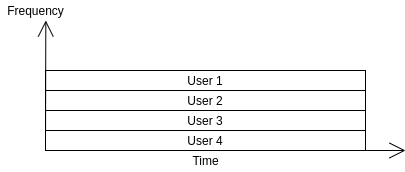
\includegraphics[width=330px]{images/1_Introduzione/FDM.png}
    \end{figure}
    
    \item Time division multiplexing:
    \begin{figure}[H]
        \centering
        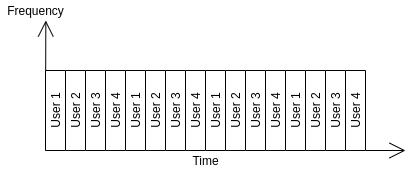
\includegraphics[width=330px]{images/1_Introduzione/TDM.png}
    \end{figure}
\end{itemize}

\subsubsection{Packet switching}
I dati che devono essere trasmessi da una parte all'altra vengono divisi in \emph{pacchetti} che sono unità di informazione all'interno della rete. Ogni pacchetto viene trasmesso usando tutta la banda del media ma solo quando c'è effettivamente la necessità di essere inviato. In alcuni casi può succedere che ci siano tanti pacchetti inviati da saturare la banda, in questi casi avviene una \emph{congestione} della rete ed i pacchetti vengono messi in coda sugli host o sui router nel mezzo in modo da essere re-inviati qualora la congestione dovesse finire. Per attuare questa commutazione si usa la tecnica dello \emph{store-and-forward} cioè si legge per intero tutto il pacchetto e lo si ri-trasmette per intero, ci si muove di hop in hop uno alla volta.

Questa tecnica di divisione del mezzo è detta \emph{statistical multiplexing} proprio perché non c'è uno scheduling preciso ma alla richiesta.


\subsubsection{Comparazione}
Il packet switching è più efficiente perché permette a molti più utenti di usare la stessa rete, inoltre è ottimo per i dati trasmessi in burst (cioè tanti pacchetti a raffica). In fine si ricordi che non c'è necessità di una \emph{chiamata} perché non va fatta una configurazione della rete.

Dall'altro lato tuttavia può soffrire di congestione che può portare a perdita di pacchetti qualora i buffer di store si riempiano.

\subsection{Packet forwarding}
Ogni pacchetto ha al suo interno un indirizzo che identifica l'host destinatario, questo indirizzo è usato dai router intermediari per indirizzare una \emph{tabella di forwarding} che associa ad ogni indirizzo di destinazione l'uscita dalla quale forwardare il pacchetto in modo che possa arrivare a termine del suo percorso.

Queste tabelle sono generate dai router stessi attraverso i protocolli di routing.

\subsubsection{Gerarchia delle reti}
Internet è una struttura gerarchica, al centro abbiamo le reti degli ISP di tier-1, questi costituiscono la \emph{backbone di internet}.
Sono reti con copertura nazionale/internazionale, tra di loro si trattano come pari proprio perché gerarchicamente lo sono.
Sono reti fortemente connesse tra di loro.

Sotto di loro abbiamo le reti degli ISP di tier-2, queste reti sono connesse ad una o più reti di tier-1, eventualmente anche ad altre reti di tier-2.
Queste reti chiedono la connessione e pagano il servizio alle reti di tier-1.
Hanno copertura regionale.

In fine ci sono le reti degli ISP di tier-3, le più piccole, a cui sono connesse le reti degli ISP locali.
Questi sono gli ISP ai quali ci si rivolge generalmente per avere connettività all'interno delle abitazioni.

Un esempio potrebbe essere:
\begin{figure}[H]
    \centering
    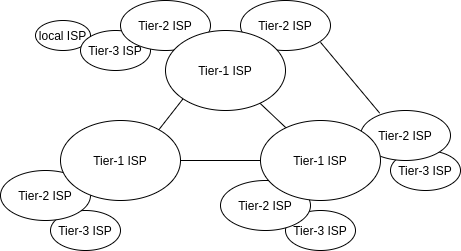
\includegraphics[width=300px]{images/1_Introduzione/hierarchy.png}
\end{figure}

Un percorso tra due host potrebbe essere:
\begin{figure}[H]
    \centering
    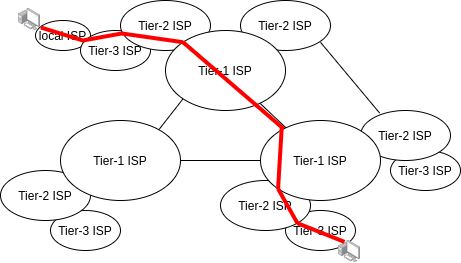
\includegraphics[width=300px]{images/1_Introduzione/path.png}
\end{figure}
Un pachetto passa attraverso tante reti e vari pacchetti tra gli stessi host non è detto che facciano la stessa strada.

NB: il tool \emph{tracert} (traceroute) è utile per vedere che percorso fa un pacchetto in quanto ci elenca tutti gli hop intermedi prima di arrivare a destinazione.

\subsubsection{Ritardi}
Abbiamo già detto che in caso di congestione potrebbero esserci delle perdite di pacchetti, diciamo che in genere la perdita o il ritardo si ha quando il rateo di arrivo eccede la capacità di output della connessione: in questi casi si crea una coda all'interno dei router intermedi che va gestita.
Abbiamo 4 sorgenti di ritardo:
\begin{figure}[H]
    \centering
    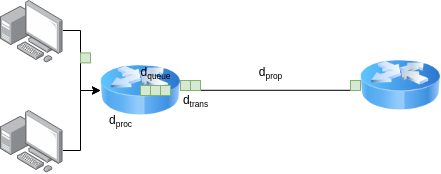
\includegraphics[width=300px]{images/1_Introduzione/delay.png}
\end{figure}

\begin{itemize}
    \item $d_{proc}$: delay di processazione, è il tempo che il router ci mette per leggere l'indirizzo di destinazione e controllare la sua forwarding table per decidere da quale uscita ritrasmettere il pacchetto
    \item $d_{queue}$: delay di accodamento, è il tempo che il pacchetto passa in coda prima che venga ritrasmesso. Questo tempo dipende fortemente da quanto la coda è lunga
    \item $d_{trans}$: delay di trasmissione, è il tempo che ci vuole per porre i singoli bit del pacchetto sul media, quindi anche il tempo per la conversione digitale/analogico. Questo tempo dipende dal media utilizzato, cioè dalla sua bandwith o bitrate.
    Dato $R$ = bandwith del link e $L$ = lunghezza del pacchetto avremo che il tempo necessario a trasmettere il pacchetto è $\frac{L}{R}$
    \item $d_{prop}$: delay di propagazione, è il tempo necessario affinché il singolo bit attraversi l'intero media. Anche questo è dipendente dal media utilizzato.
    Dato $d$ = lunghezza del media e $s$ = velocità di propagazione nel media avremo che il tempo necessario alla propagazione è $\frac{d}{s}$
\end{itemize}

Possiamo quindi dire che il delay aggiunto dal singolo nodo (hop) è:
$$ d_{nodal} = d_{proc} + d_{queue} + d_{trans} + d_{prop} $$
Se ci sono $N$ diversi nodi da attraversare il delay totale sarà la somma dei delay dei singoli nodi.

NB: Supponiamo che la banda del media sia $R$, che la lunghezza dei pacchetti sia $L$ e che $a$ sia il rateo medio di pacchetti in arrivo, allora possiamo calcolare l'intensità del traffico con: $\frac{La}{R}$.
\begin{itemize}
    \item se $\approx$ 0 il delay è approsimativamente nullo
    \item se $\approx$ 1 il delay diventa molto grande
    \item se $>$ 1 il delay cresce tendendo ad infinito. In questo caso abbiamo più pacchetti in entrata di quanti ne possiamo far uscire.
\end{itemize}

\subsubsection{Throughput}
E' il rateo al quale sono trasferiti i bit tra la sorgente e la destinazione.
Il throughput è il minore tra i bitrate dei media attraversati dal pacchetto, il collegamento avente tale bitrate è anche detto \emph{bottleneck link}.

\subsection{Network stack}
Le reti sono composte da molte componenti diverse, serve quindi una struttura standard per organizzare tutto quanto e occorre rendere compatibile e funzionante questa struttura attraverso hardware diversi, software diversi, ecc, ecc.

L'organizzazione generale delle reti prevede una pila di protocolli di astrazione sempre più crescente, ogni livello di questa pila è detto \emph{layer}.
Ogni layer fornisce un servizio seguendo un protocollo preciso e dipende dai layer precedenti.

Questa struttura a layer permette di lavorare meglio con i sistemi complessi, la manutenzione è più veloce ed efficiente sui sistemi modulari perché ogni layer è un blocco a se che espone dei servizi. A chi richiede il servizio non importa come esso sia implementato, importa solo che il servizio sia fornito.

\subsubsection{TCP/IP}
\begin{itemize}
    \item Application: ospita le applicazioni di rete
    \item Transport: si occupa del trasferimento dei dati processo-processo
    \item Network: si occupa del routing dei datagrammi dalla sorgente alla destinazione
    \item Link: si occupa del trasferimento dei dati tra elementi nella stessa rete
    \item Physical: trasmissione fisica dei bit
\end{itemize}

\subsubsection{ISO/OSI}
\begin{itemize}
    \item Application
    \item Presentation: permette all'applicazione di interpretare il significato dei dati: cifratura, compressione, ecc
    \item Session: sincronizzazione, recupero dei dati scambiati
    \item Transport
    \item Network
    \item Link
    \item Physical
\end{itemize}
Questo stack è un ampliamento di quello effettivamente utilizzato, nella pratica se questi servizi dovessero servire verrebbero implementati all'interno del layer applicativo.

\subsubsection{Incapsulamento}
Quando un host vuole inviare un messaggio deve attraversare tutti i layer fino a quello fisico:

\begin{figure}[H]
    \centering
    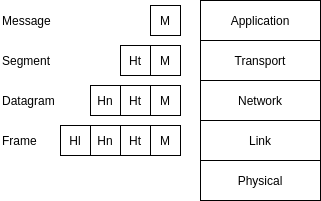
\includegraphics[width=250px]{images/1_Introduzione/encapsulation.png}
\end{figure}

Ogni layer aggiunge una nuova intestazione (header) e passa tutto al layer in basso, ogni conformazione di questo pacchetto prende un nome differente.

Alla ricezione del pacchetto i layer vengono navigati dal più basso al più alto rimuovendo tutti gli header. 


\subsection{Network security}
Il campo della sicurezza delle reti si occupa di:
\begin{itemize}
    \item come gli attori malevoli attaccano le reti
    \item come ci si può difendere da questi attacchi
    \item progettare reti e protocolli immuni
\end{itemize}

Un problema fondamentale è che Internet non è nata con criteri di sicurezza in testa in quanto all'inizio era una piccola rete ristretta a persone che si conoscevano tra di loro e quindi con una mutua fiducia, quando la rete ha iniziato ad ingrandirsi e sono apparsi i primi problemi si è ricorsi a mettere in sicurezza ciò che si poteva implementando criteri di sicurezza su tutti i layer dello stack.

Gli attacchi sulla rete prevedono sia attacchi ai singoli host della rete:
\begin{itemize}
    \item diffusione di malware attraverso virus, worm e trojan
    \item inserimento di software spyware 
    \item arruolamento all'interno di grandi botnet pensate per il DDoS (Distributed Denial of Service - negazione di servizio distribuito)
\end{itemize}
sia anche attacchi a dispositivi che compongono l'infrastruttura di rete.

Ci si può disporre all'ascolto e perpetrare un \emph{packet sniffing} cioè una cattura dei pacchetti scambiati tra vari host, per intercettare informazioni sensibili.

Si possono craftare pacchetti con ip sorgente custom per fingersi un'altra macchina: \emph{IP-spoofing}.

Si può replicare il traffico catturato per fingersi qualcun altro: \emph{reply attack}.

\subsection{Storia di Internet}
Un giorno in cui non piove tanto la scriverò